\documentclass[11pt, red]{beamer}

 %%Pacotes
\usepackage{beamerprosper}
\usepackage[utf8]{inputenc}
\usepackage[portuguese, brazilian]{babel}
\usepackage{amsmath,amsthm,amsfonts,amssymb}
\usepackage[mathcal]{eucal}
\usepackage{listings}
\usepackage{color}
\usepackage{graphicx}
\usepackage{algpseudocode}
\usepackage{algorithm2e}
    
\usepackage[alf,bibjustif]{abntex2cite}
%%%%%%%%%
%%Temas%%
%%%%%%%%%

    \mode<presentation>
    
    \useinnertheme[shadow=true]{rounded}
    \useoutertheme{infolines}
    \usecolortheme{beaver}
    
    \setbeamerfont{block title}{size={}}
    \setbeamercolor{titlelike}{parent=structure,bg=white}
    \mode
    <all>
    
    \useoutertheme{infolines}

  %%Informações para o arquivo PDF
    \hypersetup{
      pdftitle={Loteria Descentralizada em Blockchain EOSIO},
      pdfauthor={Ricardo de Barros Marli\`ere},
      pdfsubject={Blockchain},
      pdfkeywords={Bitcoin, criptomoeda, descentraliza\c{c}\~ao, blockchain, EOSIO},
    }
  %%%%%

  %%Atalhos / definições / novos comandos
    %%Atalhos para cores
      \newcommand{\verm}{\textcolor[rgb]{1.00,0.00,0.00}}
      \newcommand{\azul}{\textcolor[rgb]{0.00,0.00,1.00}}
      \newcommand{\verd}{\textcolor[rgb]{0.00,0.59,0.00}}

    %%%%%
    %%Define funções trigonométricas como texto
      \newcommand{\sen}{{\, \rm sen\,}}
    %%%%%
    %%Atalho negrito de símbolos
      \def\bs{\boldsymbol}
    %%%%%
    %%Atalho para cor dos links
      \newcommand{\corlink}{\textcolor[rgb]{0.00,0.00,1.00}}

    \definecolor{codegreen}{rgb}{0,0.6,0}
    \definecolor{codegray}{rgb}{0.5,0.5,0.5}
    \definecolor{codepurple}{rgb}{0.58,0,0.82}
    \definecolor{backcolour}{rgb}{0.95,0.95,0.95}
    

    \lstset{
    numberstyle=\color{codegray},
    numbers=left, 
    numbersep=8pt, 
    frame = single,
    framexleftmargin=0pt,
    xleftmargin=10pt,
    backgroundcolor=\color{backcolour},   
    commentstyle=\color{codegreen},
    breakatwhitespace=false,
    basicstyle=\ttfamily,
    columns=flexible,
    breaklines=true,                 
    keepspaces=true,
    showspaces=false,                
    showstringspaces=false,
    showtabs=false,                  
    tabsize=2,
    literate= {á}{{\'a}}1 {à}{{\`a}}1 {ã}{{\~a}}1 {â}{{\^a}}1 {é}{{\'e}}1 {ê}{{\^e}}1 {í}{{\'i}}1 {ó}{{\'o}}1 {õ}{{\~o}}1 {ú}{{\'u}}1 {ü}{{\"u}}1 {ç}{{\c{c}}}1 {Á}{{\'A}}1 {À}{{\`A}}1 {Ã}{{\~A}}1 {Â}{{\^A}}1 {É}{{\'E}}1 {Ê}{{\^E}}1 {Í}{{\'I}}1 {Ó}{{\'O}}1 {Õ}{{\~O}}1 {Ú}{{\'u}}1 {Ç}{{\c{C}}}1
    }  

    %%%%%
  %%%%%
%%%%%%%%%%%%%%%%%%%%%
%% Novos ambientes %%
%%%%%%%%%%%%%%%%%%%%%
  \newtheorem{teor}{Teorema}%[section]
  \newtheorem{resu}{Resultado}%[section]
  \newtheorem{lema}{Lema}%[section]
  \newtheorem{prop}{Proposição}%[section]
  \newtheorem{defi}{Definição}%[section]
  \newtheorem{exem}{Exemplo}%[section]
  \newtheorem{exer}{Exercício}%[section]
%%%%%
%%%%%
%%%%%%%%%%%%%%%%%%%%%%%%%%%%%%%%%%%%%%%%%%%%%%%%%%%%%%%%%%%%%
%% Configurações de ambientes (teoremas, exemplos, etc...) %%
%%%%%%%%%%%%%%%%%%%%%%%%%%%%%%%%%%%%%%%%%%%%%%%%%%%%%%%%%%%%%
\setbeamertemplate{theorem begin}{{\textup{\structure{\textbf{\underline{\inserttheoremname
\inserttheoremnumber \if \ \inserttheoremaddition \else \ \inserttheoremaddition \fi:}~}}}}}
\setbeamertemplate{theorem end}
%%%%%
%%%%%
%%%%%%%%%%%%%%%%%%%%%%%%%%%%%%%%%%%%%%%
%% Configurações das caixas de texto %%
%%%%%%%%%%%%%%%%%%%%%%%%%%%%%%%%%%%%%%%
  \beamertemplatetransparentcovereddynamic
  \beamerboxesdeclarecolorscheme{alert}{black!20!blue!60!} {blue!10!averagebackgroundcolor}
\colorlet{cinzaLeve}{gray!10} % definindo cor
\setbeamercolor{fundocinza}{fg=black,bg=cinzaLeve} % definindo cor para bloco
\setbeamercolor{fundovermelho}{fg=white,bg=structure} % definindo cor para bloco
\setbeamercolor{fundoazul}{fg=black,bg=blue!30} % definindo cor para bloco
\setbeamercolor{fundobranco}{fg=black,bg=white} % definindo cor para bloco
%%%%%
%%%%%
%%%%%%%%%%%%%%%%%%%%%%%%%%%%%%%%%%%%%%%%%%%%%%%%%%%%%%%%
%%%%%%%%%%%%%%%%%%%%%%%%%%%%%%%%%%%%%%%%%%%%%%%%%%%%%%%%



%%%%%%%%%%%%%%%%%%%%%%%%%%%%%%%%%%%%
%% Configurações do slide inicial %%
%%%%%%%%%%%%%%%%%%%%%%%%%%%%%%%%%%%%

  \title[Loteria em EOSIO]{\large{Loteria Descentralizada em Blockchain EOSIO} }

  \author[Ricardo de Barros Marli\`ere]{
    {\small \textcolor[rgb]{0.00,0.00,0.63}{\textit{ \ }}}\\
    \vspace{0.2cm}
    {\small \textcolor[rgb]{0.00,0.00,0.63}{\textit{ \ }}}\\
    {\color{black} \text{} }\\
    {\color{black} Ricardo de Barros Marli\`ere }\\
    {\color{black} \ }\\
  }

  \institute[UFJF]{Universidade Federal de Juiz de Fora}

  \date{Dezembro de 2018}

%%%%%%%%%%%%%%%%%%%%%%%%%%%%%%%%%%%%%%%%%%%%%%%%%%%%%%%%
%%%%%%%%%%%%%%%%%%%%%%%%%%%%%%%%%%%%%%%%%%%%%%%%%%%%%%%%

\begin{document}

%%%%%%%%%%%%%%%%%%%%%%%%%%%%%%%
%% Exibição do slide inicial %%
%%%%%%%%%%%%%%%%%%%%%%%%%%%%%%%

\begin{frame}[plain]
    \titlepage
\end{frame}

%%%%%%%%%%%%%%%%%%%%%%%%%%%%%%%
%%%%% Conteúdo dos slides %%%%%
%%%%%%%%%%%%%%%%%%%%%%%%%%%%%%%

%%%%%%%%%%%%%%%%%%%%%%%%%%%%%%%
\section[ ]{Introdu\c{c}\~{a}o}
%%%%%%%%%%%%%%%%%%%%%%%%%%%%%%%

%%%%%%%%%%%%%%%%%%%%%%%%%%%%%%%
\subsection[Introdu\c{c}\~{a}o]{Introdu\c{c}\~{a}o}

\begin{frame}
    \frametitle{Hist\'{o}rico}
        \begin{columns}
        \scriptsize
        \column{0.3\textwidth}
        \begin{figure}[htb]
            \begin{center}
                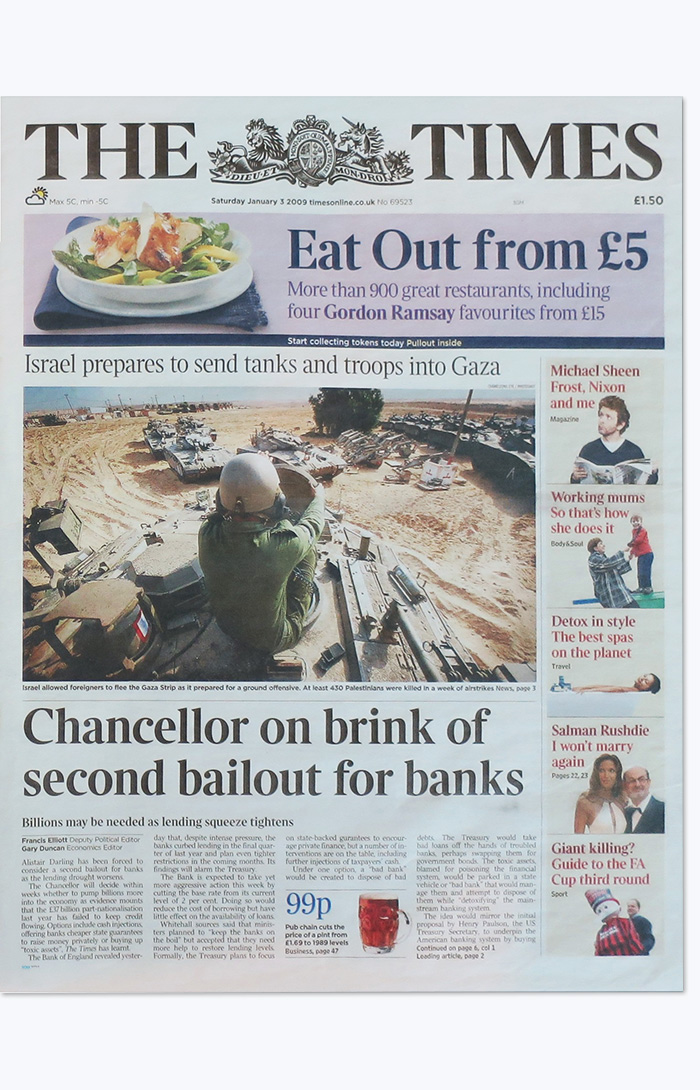
\includegraphics[width=1.2\linewidth]{fig/genesis.jpg}
            \end{center}
        \end{figure}
        \column{0.7\textwidth}
            \begin{itemize}
            	\item Bitcoin \'{e} concebido em 2008 e implementado em 2009.
                \item Ethereum \'{e} concebido em 2013 e implementado em 2015.
                \item EOSIO \'{e} concebido em 2017 e implementado em 2018.
            \end{itemize}
        \end{columns}
\end{frame}

\begin{frame}
    \frametitle{Problema de Plataformas Centralizadas}
    \begin{beamerboxesrounded}[lower=fundocinza,shadow=true]{}
        \begin{columns}
        \scriptsize
        \column{0.5\textwidth}
        \begin{figure}[htb]
            \begin{center}
                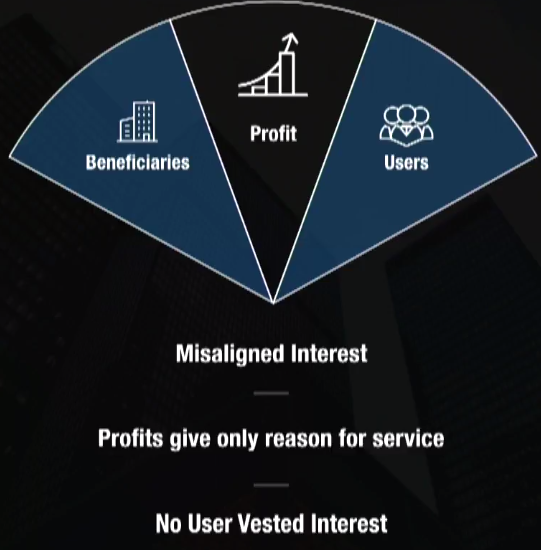
\includegraphics[width=0.9\linewidth]{fig/mitm.png}
            \end{center}
        \end{figure}
        \column{0.5\textwidth}
            Exemplos:
            \begin{itemize}
                \item Uber n\~ao possui carros.
                \item Airbnb n\~ao possui im\'oveis.
                \item Spotify n\~ao cria m\'usica.
                \item Facebook n\~ao cria conte\'udo.
                \item Alibaba n\~ao possui estoque.
                \item iFood n\~ao produz alimentos.
            \end{itemize}
        \end{columns}
    \end{beamerboxesrounded}
\end{frame}

\begin{frame}
    \frametitle{Objetivo das Blockchains}
    \framesubtitle{Descentralizar e remover intermedi\'arios}
    \begin{figure}[htb]\label{ex1}
        \begin{center}
            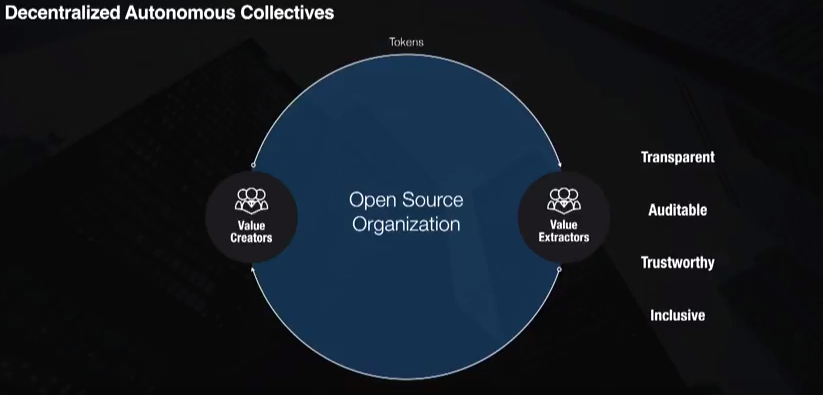
\includegraphics[width=1\linewidth]{fig/dac.png}
        \end{center}
    \end{figure}
\end{frame}

%%%%%%%%%%%%%%%%%%%%%%%%%%%%%%%
\subsection[Fundamenta\c{c}\~{a}o Te\'{o}rica]{Fundamenta\c{c}\~{a}o Te\'{o}rica}

\begin{frame}
    \frametitle{Blockchain}
    \framesubtitle{Transfer\^encia de Propriedade}
    \begin{figure}[htb]\label{ex1}
        \begin{center}
            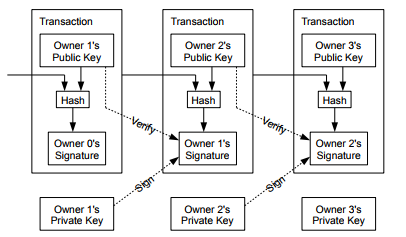
\includegraphics[width=0.5\linewidth]{fig/btc1.png}
        \end{center}
    \end{figure}
    \begin{beamerboxesrounded}[lower=fundocinza,shadow=true]{}
        \begin{itemize}
        	\item Dono anterior anuncia o novo dono.
            \item Prova-se criptograficamente que num determinado momento (bloco) a propriedade foi alterada.
            \item Assim, o dono anterior n\~ao consegue gastar as mesmas moedas novamente.
        \end{itemize}
    \end{beamerboxesrounded}
\end{frame}

\begin{frame}
    \frametitle{Blockchain}
    \framesubtitle{Lista Encadeada de Blocos}
    \begin{figure}[htb]\label{ex1}
        \begin{center}
            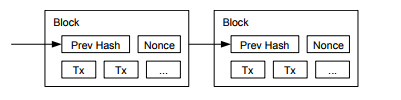
\includegraphics[width=0.6\linewidth]{fig/btc2.png}
        \end{center}
    \end{figure}
    \begin{beamerboxesrounded}[lower=fundocinza,shadow=true]{}
        \begin{itemize}
        	\item Mant\'em um livro-raz\~ao com o timestamp de cada transa\c{c}\~ao.
            \item Registro \'e mantido irrevers\'ivel por via de Proof of Work.
            \item Retrabalho para alterar o hist\'orico \'e invi\'avel.
        \end{itemize}
    \end{beamerboxesrounded}
\end{frame}
    
\begin{frame}
    \frametitle{Blockchain}
    \framesubtitle{Minera\c{c}\~ao e Proof-of-Work}
    \begin{figure}[htb]
        \begin{center}
            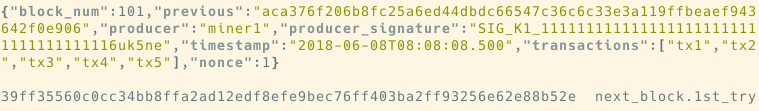
\includegraphics[width=0.8\linewidth]{fig/btc3.png}
        \end{center}
    \end{figure}
    \begin{figure}[htb]
        \begin{center}
            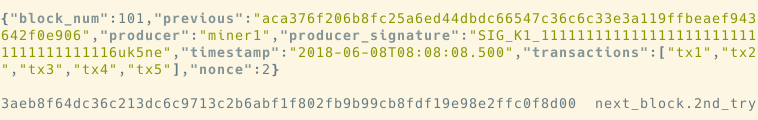
\includegraphics[width=0.8\linewidth]{fig/btc4.png}
        \end{center}
    \end{figure}
    \begin{beamerboxesrounded}[lower=fundocinza,shadow=true]{}
        \begin{itemize}
        	\item Por defini\c{c}\~ao, primeira transa\c{c}\~ao bota em circula\c{c}\~ao novas moedas para quem o descobriu.
        	\item Oferta limitada em 21 milh\~oes, emitida de forma descentralizada.
        	\item Recompensa incentiva n\'os e evita que se tornem bizantinos.
        \end{itemize}
    \end{beamerboxesrounded}
\end{frame}

\begin{frame}
    \frametitle{Smart Contracts}
    \begin{beamerboxesrounded}[lower=fundocinza,shadow=true]{}
        \begin{columns}
        \scriptsize
        \column{0.3\textwidth}
        \begin{figure}[htb]
            \begin{center}
                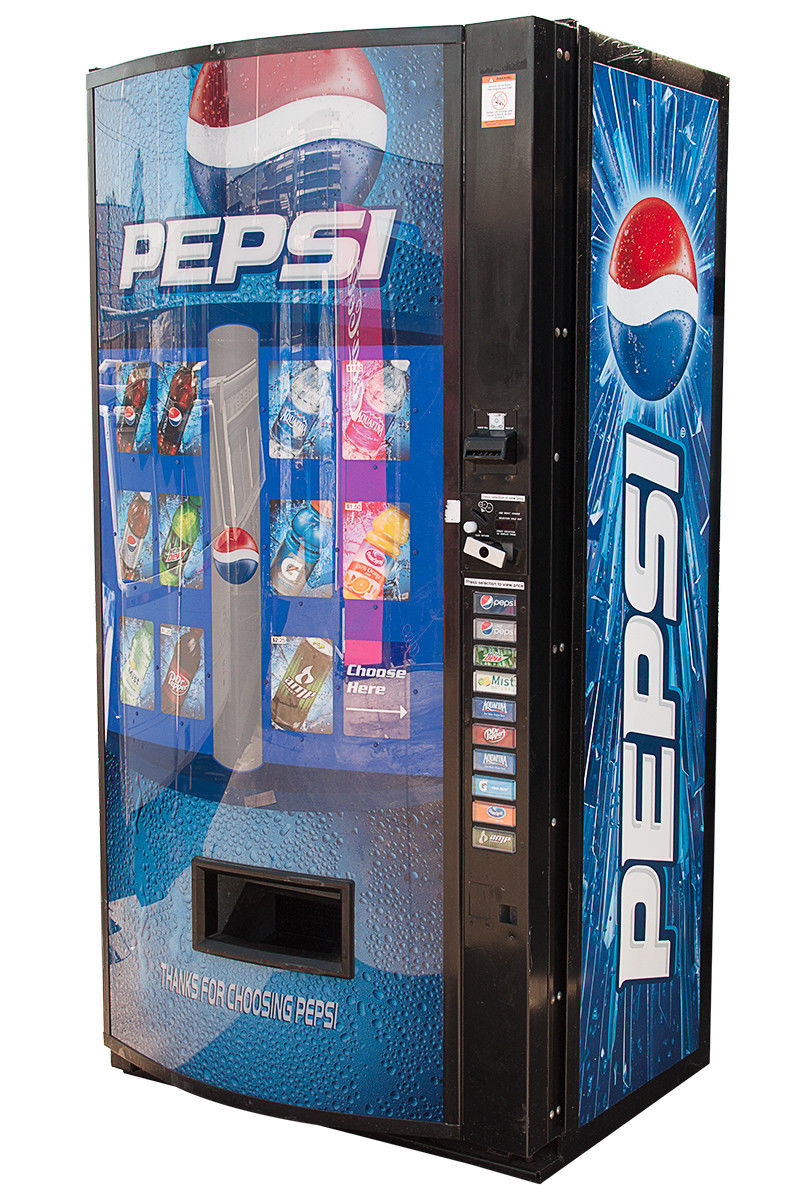
\includegraphics[width=1\linewidth]{fig/vendingmachine.jpg}
            \end{center}
        \end{figure}
        \column{0.7\textwidth}
            \begin{itemize}
            	\item Conceito concebido na d\'{e}cada de 90 e incorporado em blockchains com o advento do Bitcoin.
                \item Cl\'{a}usulas contratuais podem ser embutidas em hardware ou software, de forma a automatizar e garantir sua execu\c{c}\~{a}o.
                \item Um contrato inteligente \'e um programa cuja execu\c{c}\~ao \'e aut\^onoma, transparente e imut\'avel.
            \end{itemize}
        \end{columns}
    \end{beamerboxesrounded}
\end{frame}

\begin{frame}
    \frametitle{Smart Contracts}
        \begin{figure}[htb]
            \begin{center}
                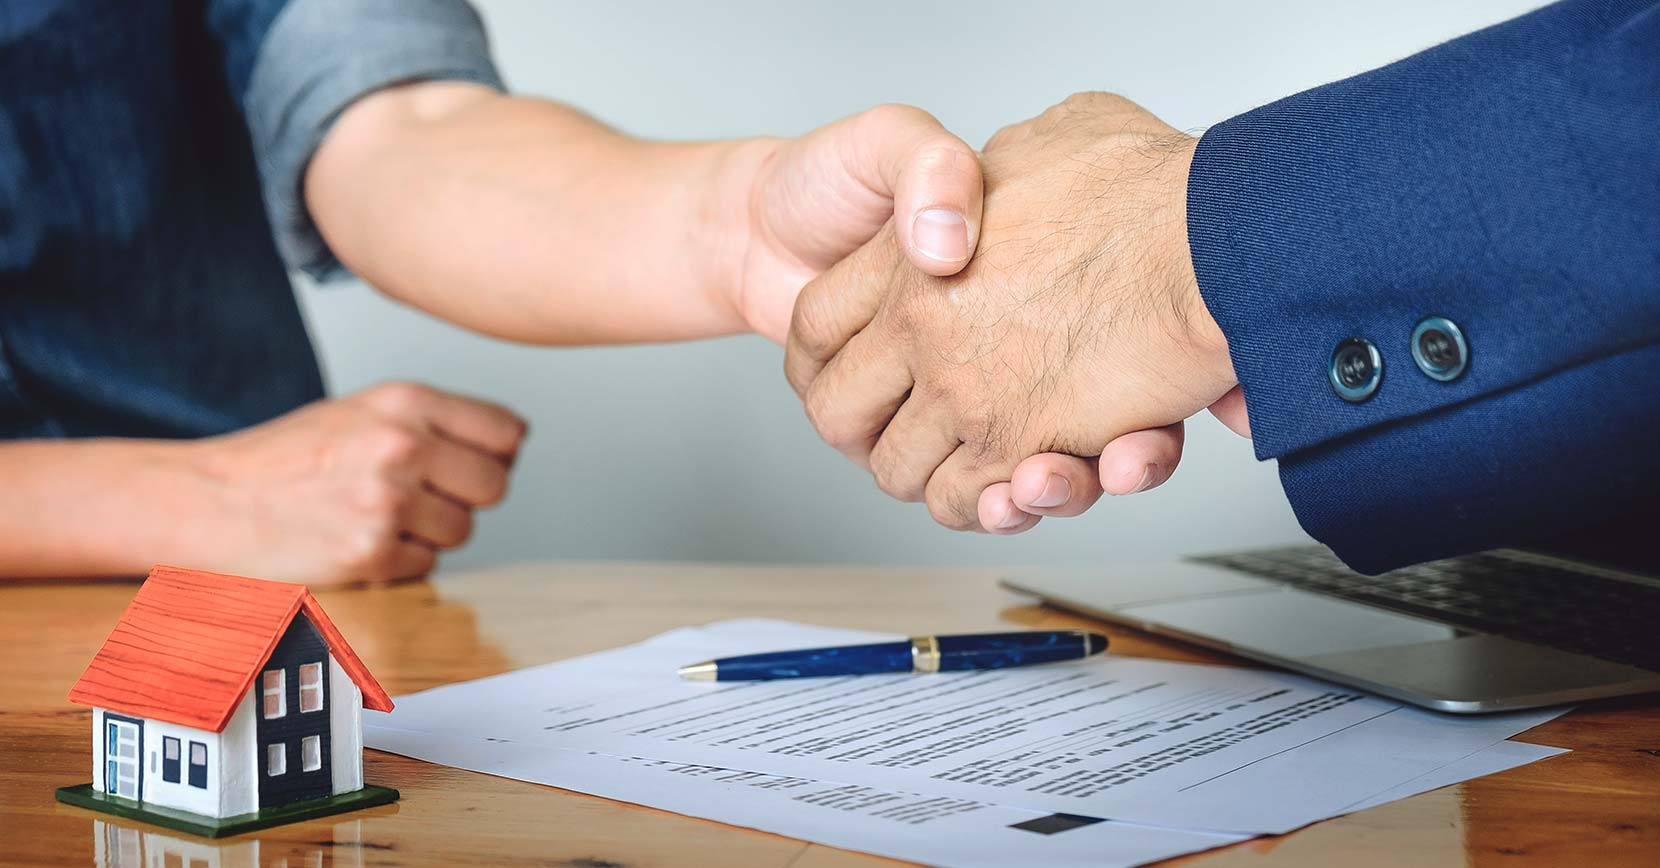
\includegraphics[width=0.5\linewidth]{fig/contrato.jpg}
            \end{center}
        \end{figure}
    \begin{beamerboxesrounded}[lower=fundocinza,shadow=true]{}
            \begin{itemize}
            	\item Um contrato "tradicional" \'e definido em papel.
                \item Leis pr\'evias existem para que sua execu\c{c}\~ao seja garantida, caso contr\'ario deve haver ju\'izo.
                \item A auditoria deve ser feita (semi) manualmente, atrav\'es da recole\c{c}\~ao de dados.
            \end{itemize}
    \end{beamerboxesrounded}
\end{frame}

\begin{frame}
    \frametitle{Smart Contracts}
    \begin{beamerboxesrounded}[lower=fundobranco]{}
        \begin{columns}
        \scriptsize
        \column{0.6\textwidth}
        \begin{figure}[htb]
            \begin{center}
                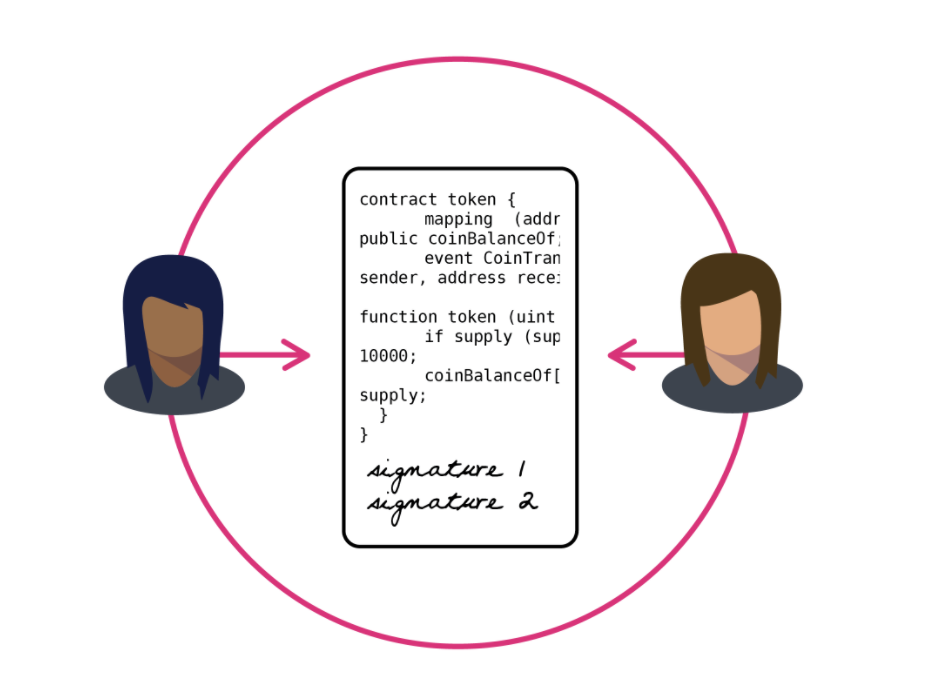
\includegraphics[width=1.2\linewidth]{fig/smartcontract.png}
            \end{center}
        \end{figure}
        \column{0.4\textwidth}
            \begin{itemize}
            	\item Um contrato inteligente \'e definido em software.
                \item Sua execu\c{c}\~ao \'e feita de consensualmente pelos n\'os validadores e suas entradas e sa\'idas tornam-se imut\'aveis.
                \item A auditoria \'e automatizada visto que os dados ficam transparentemente dispon\'iveis.
            \end{itemize}
        \end{columns}
    \end{beamerboxesrounded}
\end{frame}

%%%%%%%%%%%%%%%%%%%%%%%%%%%%%%%
\subsection[Solu\c{c}\~ao Proposta]{Solu\c{c}\~ao Proposta}

\begin{frame}
    \frametitle{Contratos em EOSIO}
    \framesubtitle{Hello World!}
    \begin{figure}[htb]\label{ex1}
        \begin{center}
            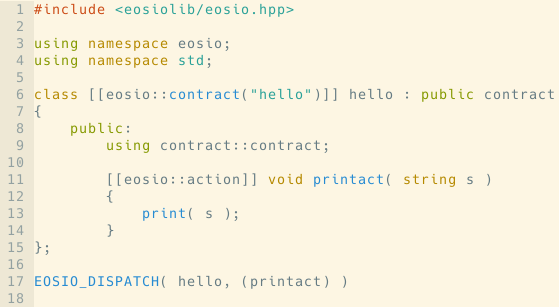
\includegraphics[width=0.7\linewidth]{fig/contract1.png}
        \end{center}
    \end{figure}
\end{frame}

\begin{frame}
    \frametitle{Contratos em EOSIO}
    \framesubtitle{Implanta\c{c}\~ao}
    \begin{figure}[htb]\label{ex1}
        \begin{center}
            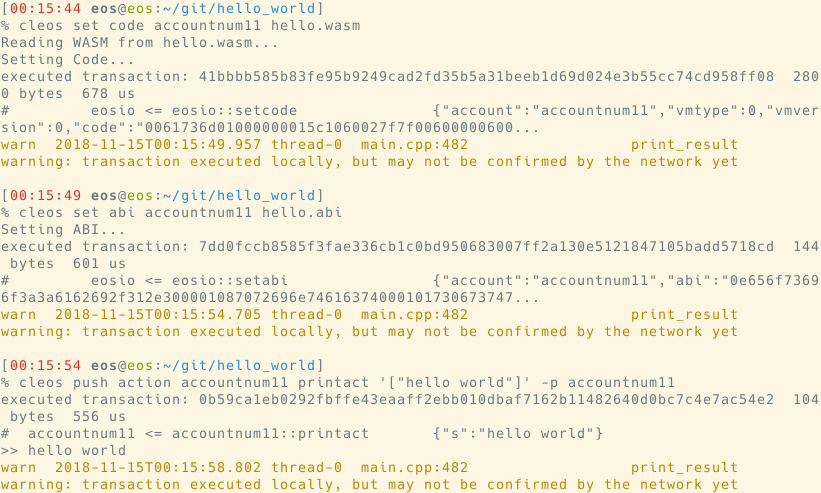
\includegraphics[width=0.9\linewidth]{fig/contract2.png}
        \end{center}
    \end{figure}
\end{frame}

\begin{frame}
    \frametitle{Objetivo do Trabalho}
    \framesubtitle{Descentralizar uma Loteria}
    \begin{figure}[htb]
        \begin{center}
            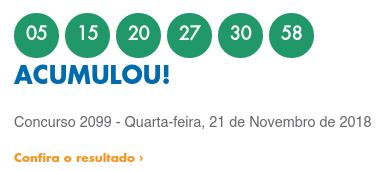
\includegraphics[width=0.5\linewidth]{fig/mega.png}
        \end{center}
    \end{figure}
    \begin{beamerboxesrounded}[lower=fundocinza,shadow=true]{}
            \begin{itemize}
                \item Ao inv\'es de depender de "Caminh\~oes da Sorte", programa-se um contrato para gerenciar as apostas e escolher os vencedores.
                \item Usu\'arios interagem com o contrato atrav\'es de chamadas criptograficamente autorizadas \`as suas a\c{c}\~oes.
            \end{itemize}
    \end{beamerboxesrounded}
\end{frame}

\begin{frame}
    \frametitle{Modelo da Aplica\c{c}\~ao}
    \framesubtitle{Fluxo do Jogo}
    \begin{figure}[htb]\label{ex1}
        \begin{center}
            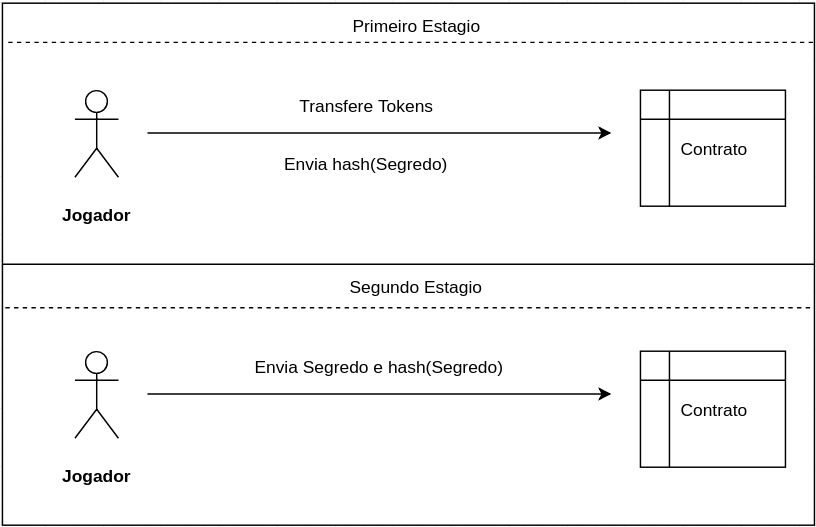
\includegraphics[width=0.8\linewidth]{fig/flow.png}
        \end{center}
    \end{figure}
\end{frame}

\begin{frame}
    \frametitle{Modelo da Aplica\c{c}\~ao}
    \framesubtitle{A\c{c}\~oes do Contrato}
    \begin{figure}[htb]\label{ex1}
        \begin{center}
            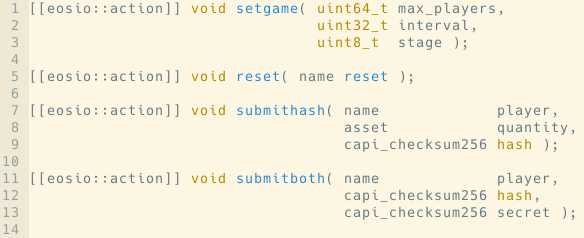
\includegraphics[width=0.8\linewidth]{fig/contract3.png}
        \end{center}
    \end{figure}
\end{frame}

\begin{frame}
    \frametitle{Modelo da Aplica\c{c}\~ao}
    \framesubtitle{Tabelas do Contrato}
    \begin{figure}[htb]\label{ex1}
        \begin{center}
            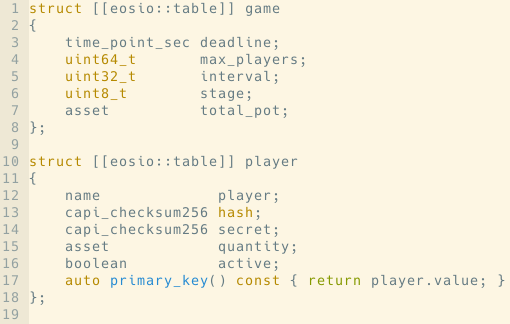
\includegraphics[width=0.7\linewidth]{fig/contract4.png}
        \end{center}
    \end{figure}
\end{frame}

\end{document}